\chapter{Implementation Plan}
%Self-propelled arrangement of and conduct at project meetings. Setting agendas and work plans.
%Appropriate self-driven use of supervisor(or other people) as source of information and advice.

\section{Milestones}
In order to tackle this robot manipulation of shoelaces problem, the project is divided into 4 stages, each has corresponding deliverables used to track the whole project. Researches and experiments of the next stage will base on the success of the previous stage. Moreover, there are some compulsory project deliverables. To be specific, they are Inception Report, Interim Report (28/01/2019), Abstract (03/06/2019), Final Report (19/06/2019) and Presentation (End of June 2019). Each deliverable and its expected time to complete is listed below.


\begin{figure}[h!]
    \centering
    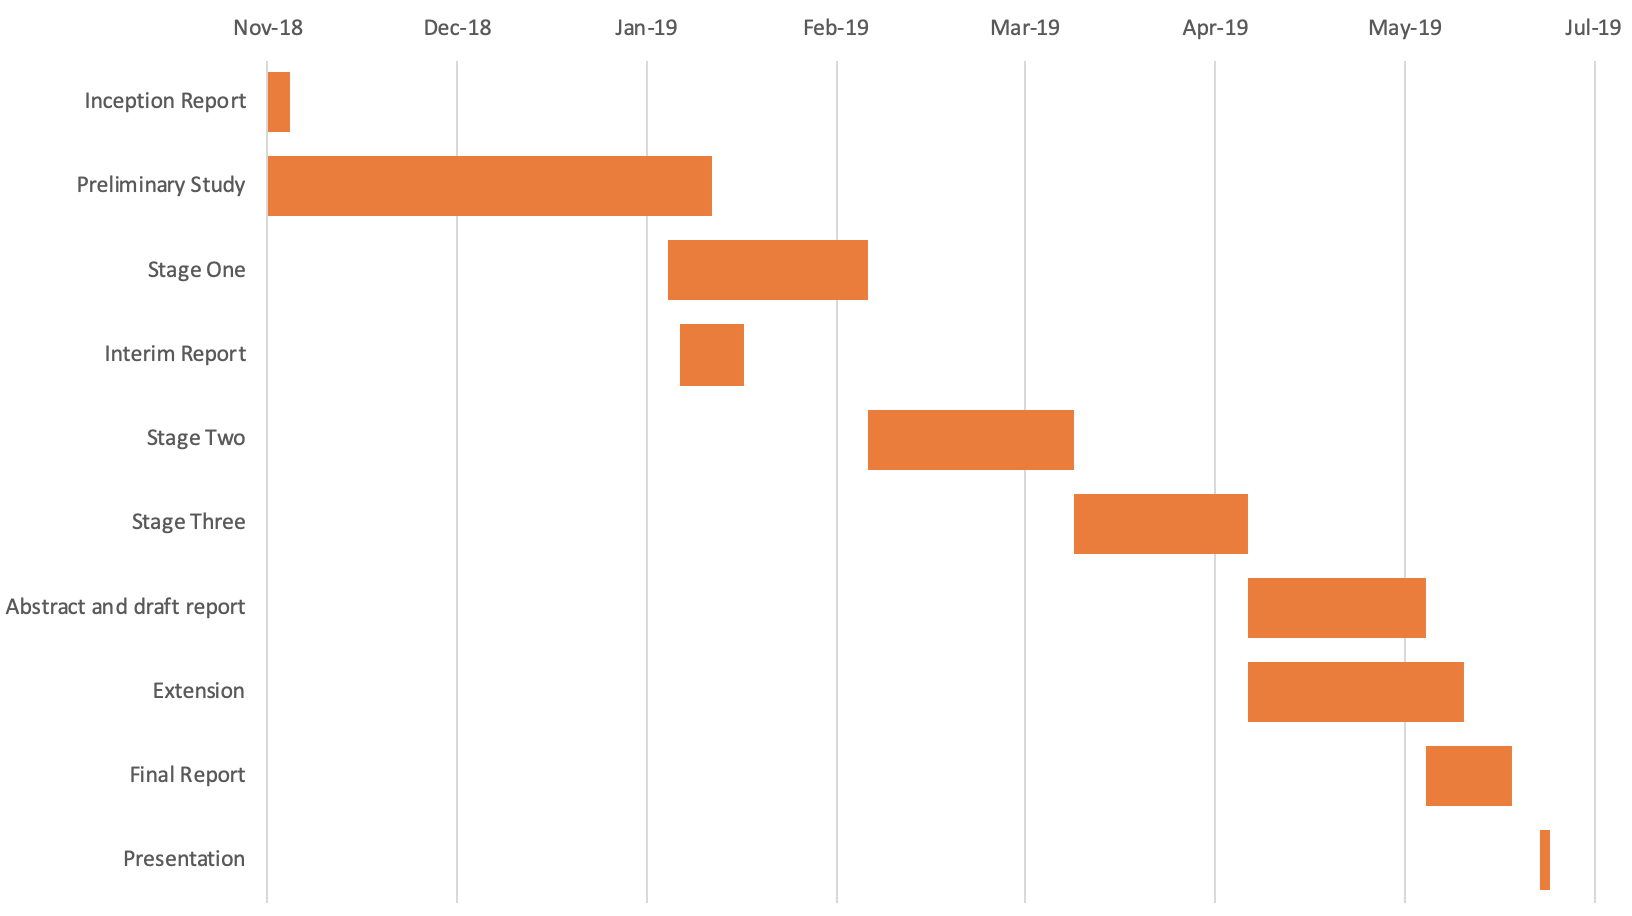
\includegraphics[width = 1\columnwidth]{images/gantt_chart.png}
    \caption{Project Gantt Chart}
\end{figure}

\begin{itemize}
  \item Stage 1: Starting with one arm holding one end of the shoelace, YuMi should detect one of the shoe holes and be able to put the shoelace into that hole. (By February 2019)
  \item Stage 2: After one arm putting the shoelace into the hole, the other arm should locate this shoelace and pull it out to complete this single hole. (By March 2019)
  \item Stage 3: Based on the success of the first 2 stages, YuMi should be able to plan sequences of robot arm trajectories for completing the whole shoe. (By May 2019)
  \item Stage 4 - Extension (By June 2019)
   \begin{enumerate}
    \item If everything goes smoothly, this project will combine with the project Robot manipulation of Shoelaces – Vision: Detection, Representation and Tracking. The success of the combination will allow YuMi to detect and pick up a shoelace from the table, then putting the shoelace on a shoe. 
    \item Another extension of this project is to optimize the performance of the robot, such as using a shoe with smaller shoe holes as the experimental subjects, or speeding up the whole operation process etc. 
  \end{enumerate}
\end{itemize}

\section{Stage One}

\begin{figure}[h!]
    \centering
    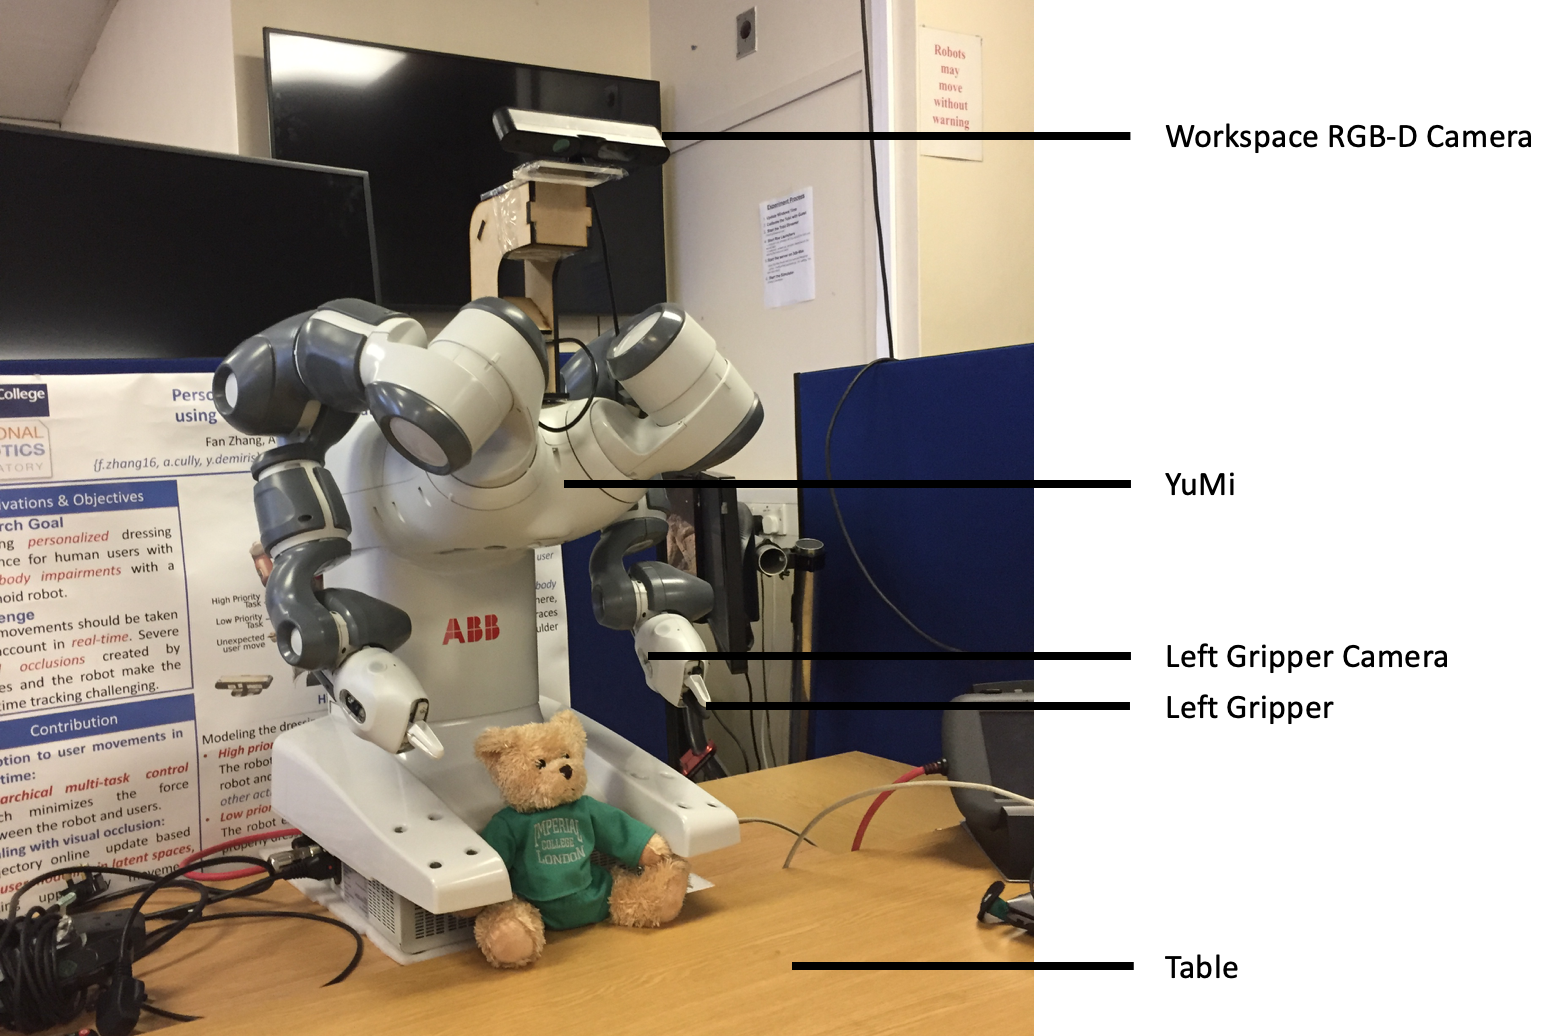
\includegraphics[width = 0.8\columnwidth]{images/yumi1.png}
    \caption{Robot platform consisting of robot YuMi and a RGB-D camera}
\end{figure}

%Report summarises past project work as completed tasks. 
The approaches to implementing stage one comprise the following steps.
\begin{itemize}
 \item Using the workspace camera, detect the shoe on the table. If no object is found, YuMi remains stationary.
 \item YuMi gripper is then positioned above the detected shoe and being closet to the centroid of it. 
 \item Using the gripper camera to view the shoe holes and calculate the precise location of one hole.
 \item YuMi plans a motion to pass the shoelaces into that hole.
\end{itemize}

Several object detection methods have been discussed in the background chapter. The first method I implemented is color detection, which has been tested on a shoe (Figure \ref{shoe}) and a shoelace (Figure \ref{shoelace}). The algorithm first converts RGB images obtained from Kinect camera to HSV colorspace, then extracts all areas whose color are within the predefined range. Currently, the interested color is set to blue. If an extracted area exceeds a predefined threshold value, then this area will be regarded as an object and its centroid 2D coordinate will be calculated. The algorithm will be updated soon to obtain the corresponding real-world 3D location. 
%-----------------------
\begin{figure}[H]
\centering
%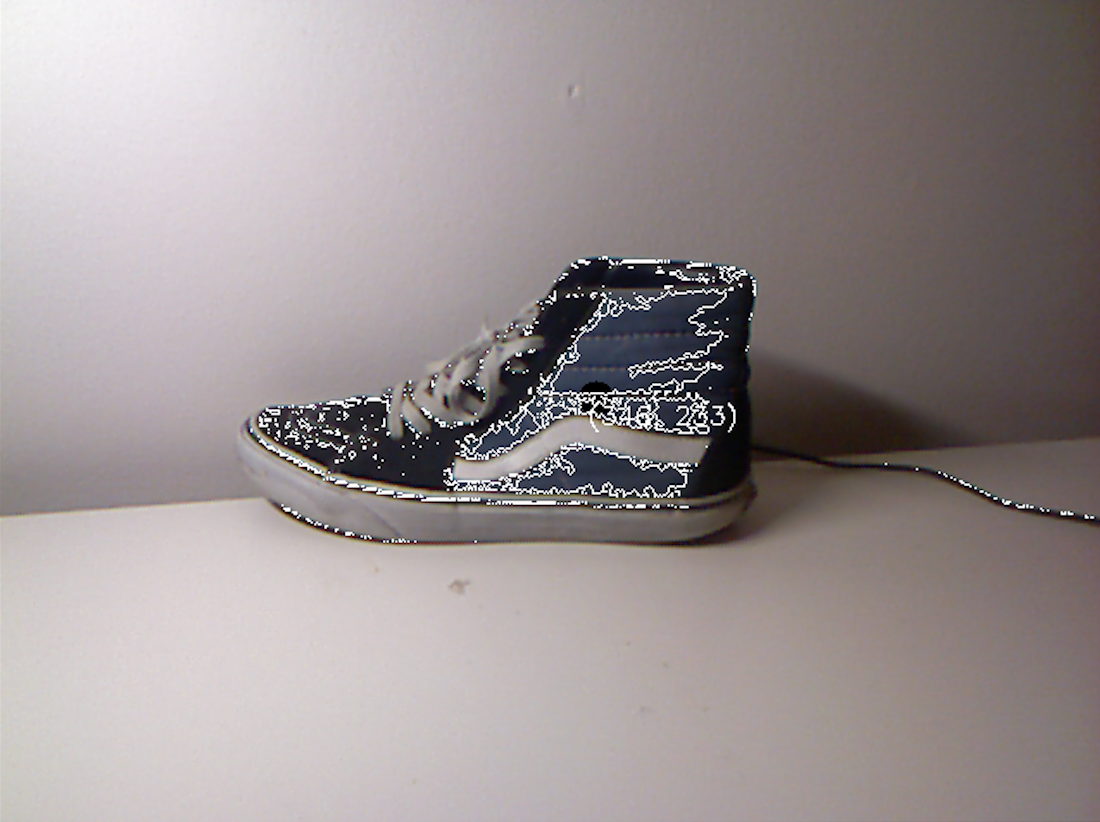
\includegraphics[width = 0.3\columnwidth]{images/1_1.png}
%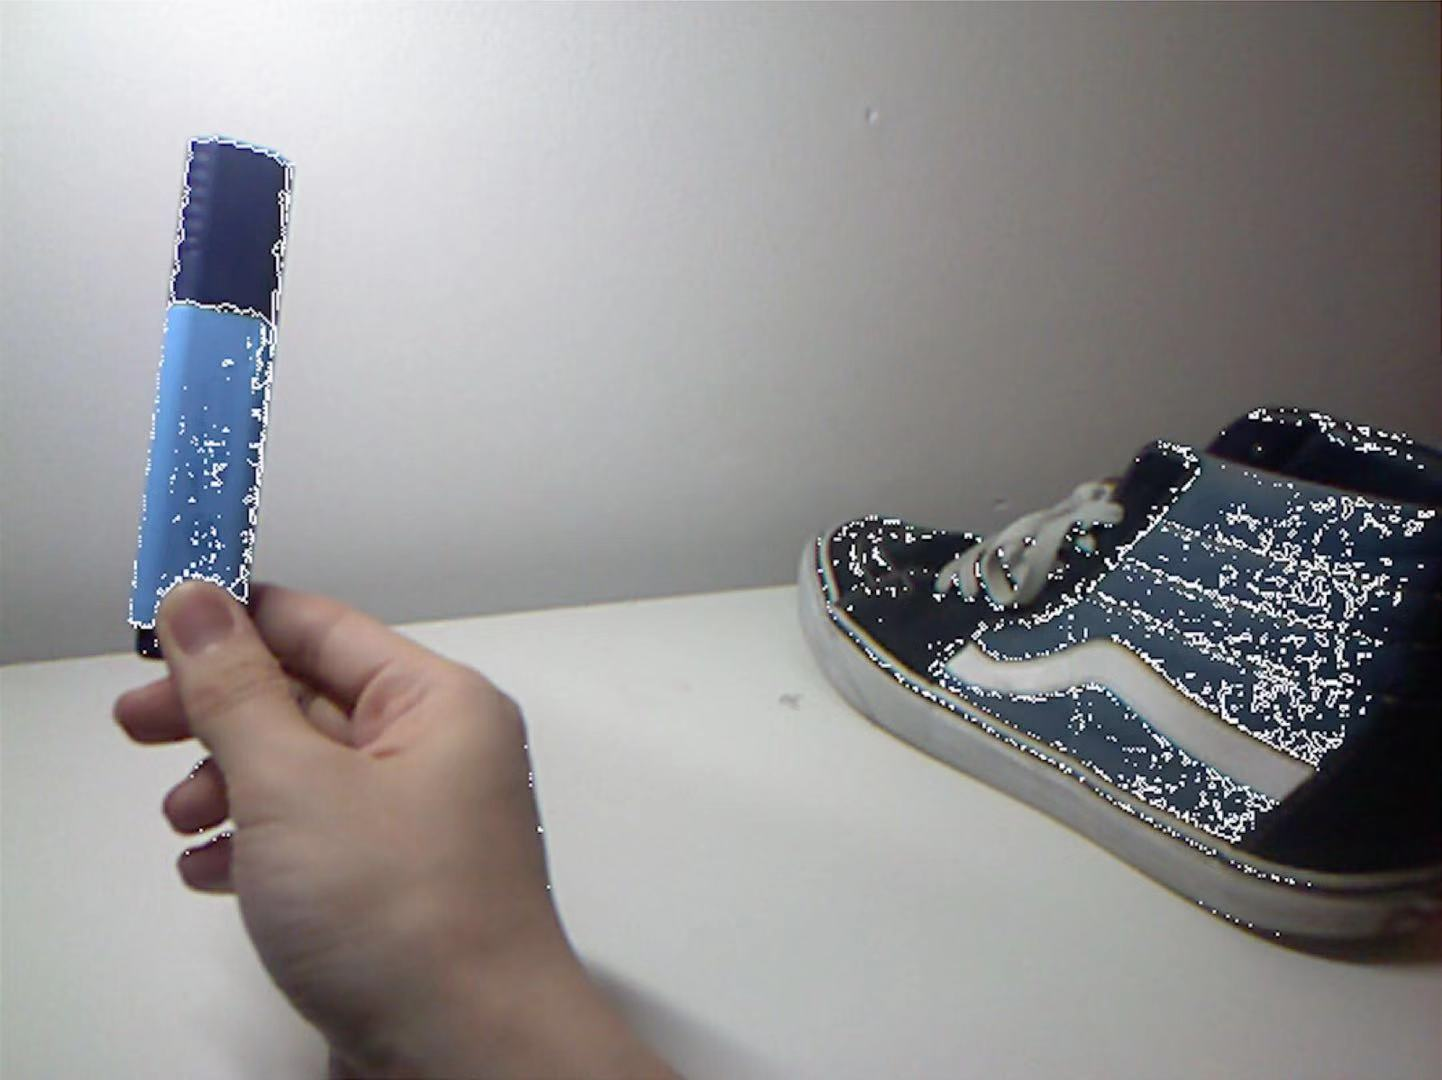
\includegraphics[width = 0.3\columnwidth]{images/2_1.png}
%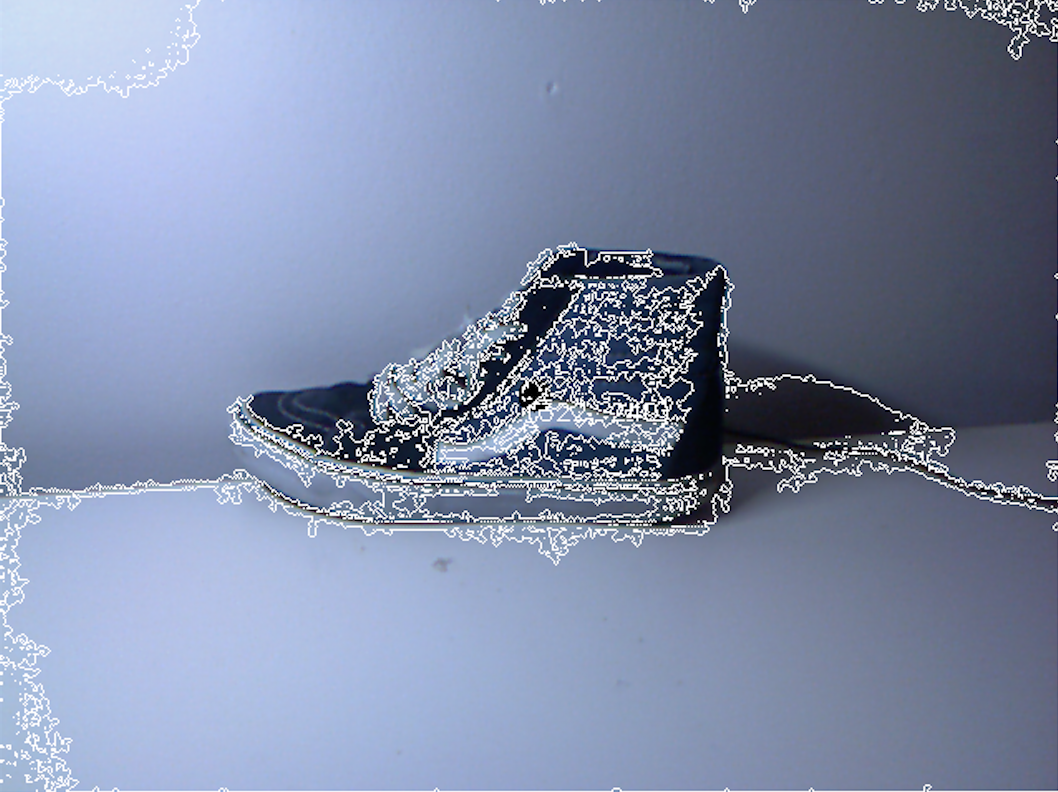
\includegraphics[width = 0.3\columnwidth]{images/3_1.png}
\subfigure[normal light]{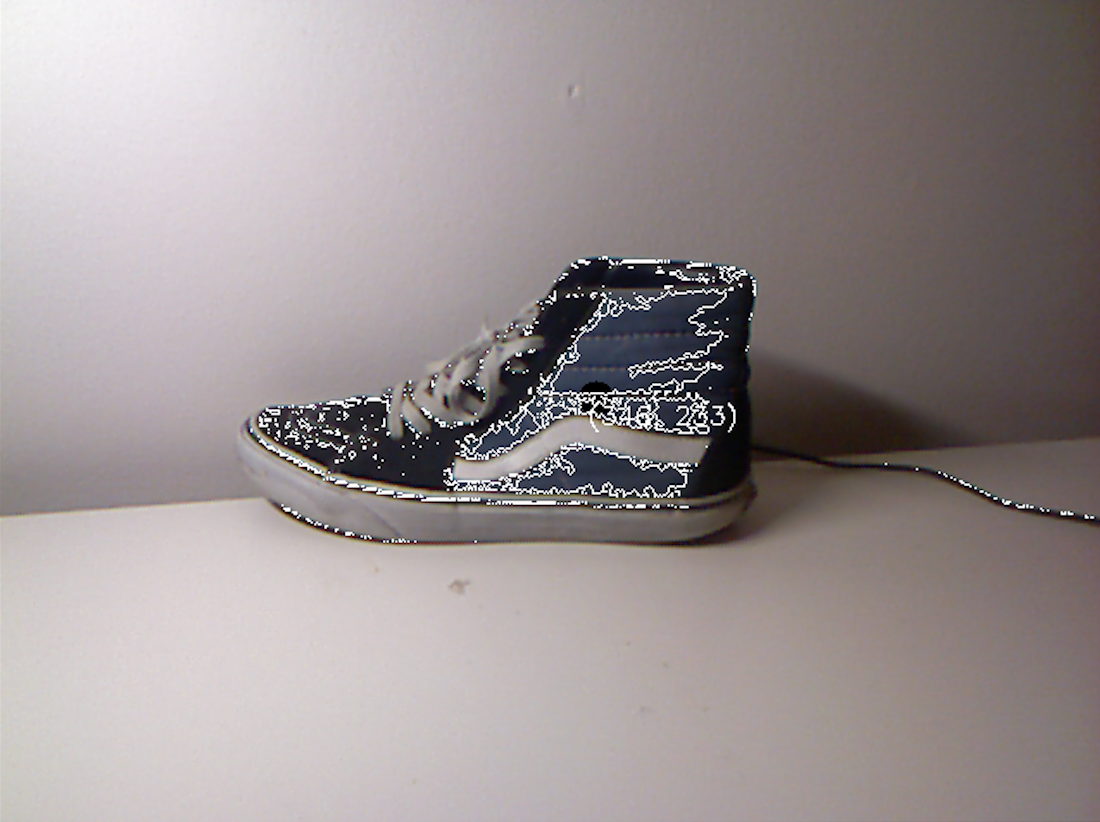
\includegraphics[width = 0.33\columnwidth]{images/1_1.png}}%
\subfigure[two blue objects]{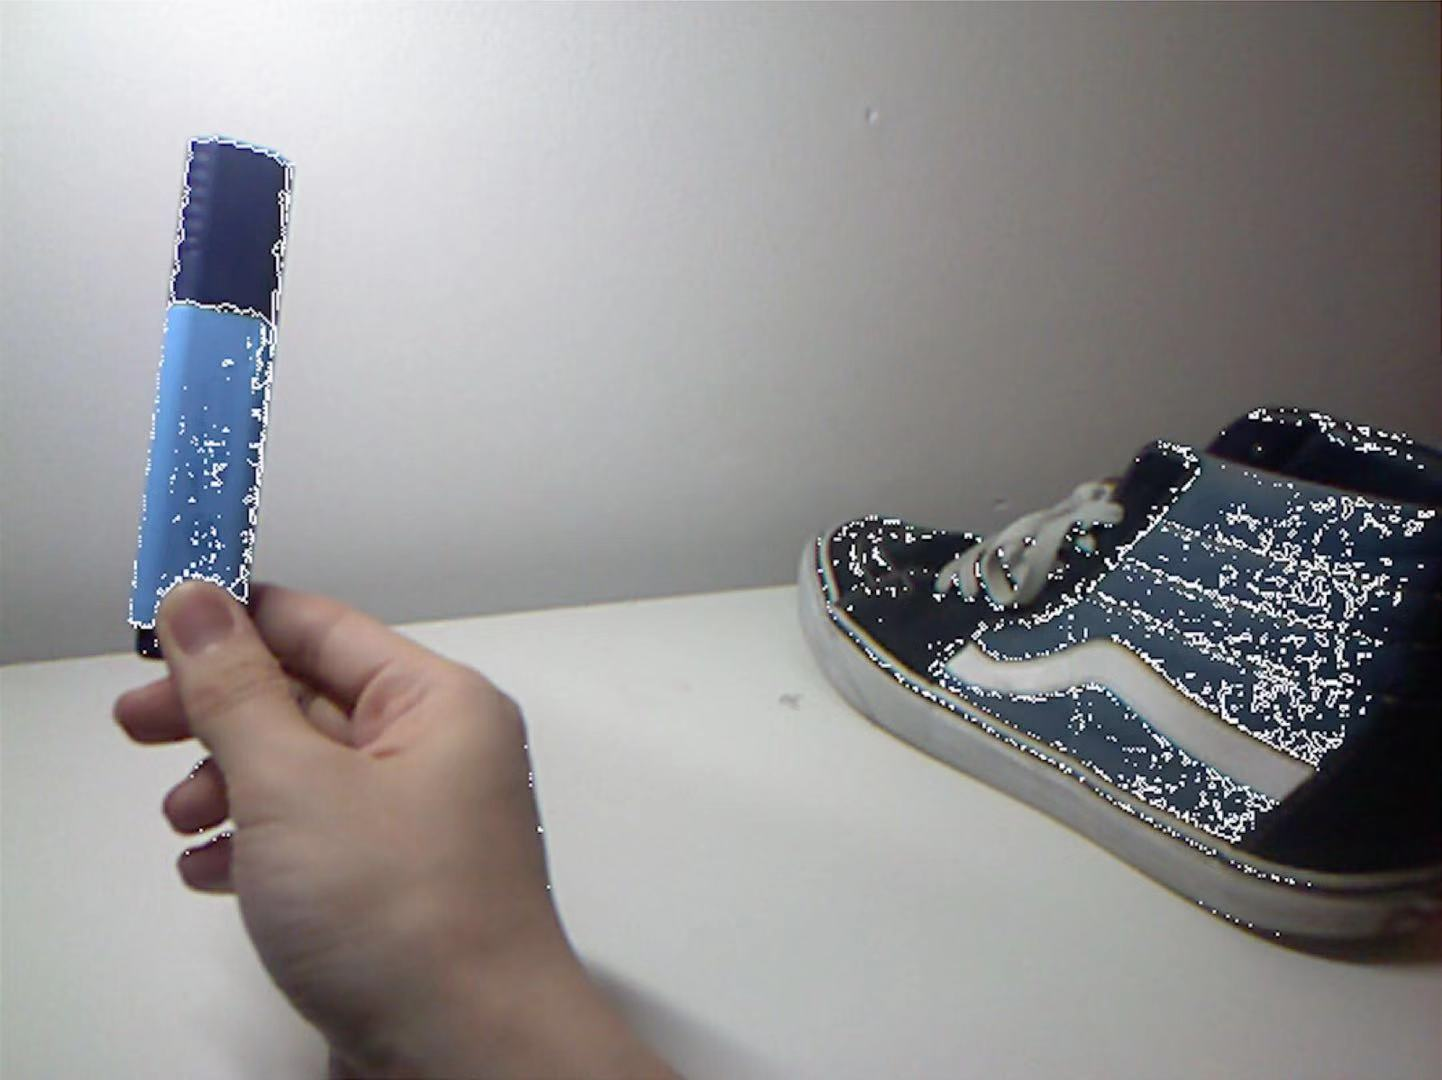
\includegraphics[width = 0.33\columnwidth]{images/2_1.png}}%
\subfigure[cold light]{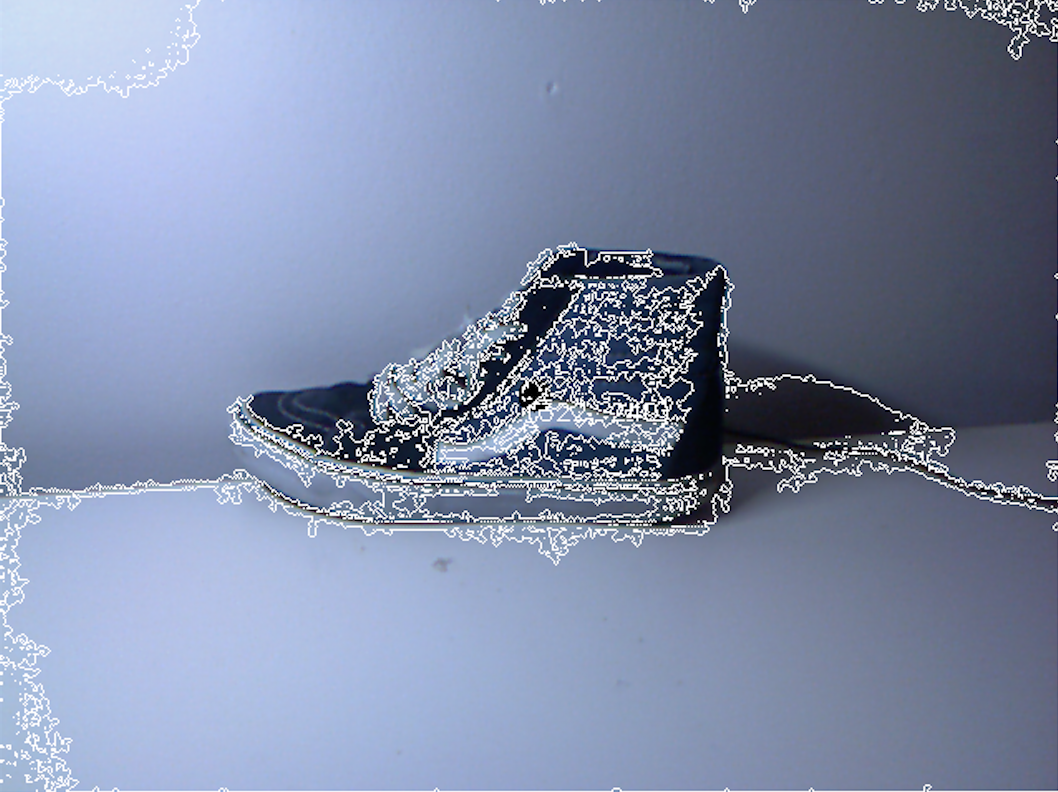
\includegraphics[width = 0.33\columnwidth]{images/3_1.png}}%
\caption{Color detection algorithm testing on a shoe in different environments}%
\label{shoe}%
\end{figure}
%-----------------------
In the normal light environment, the shoe can be correctly detected by Kinect camera. However, blue is a cold color, when putting the shoes under cold light, almost all the detected areas were recognized as the object. Furthermore, when there are more than one blue objects, the algorithm has no idea which one should be chosen. Overall, using this detection method to locate a shoe on a table is not reliable.
%-----------------------
\begin{figure}[H]
\centering
%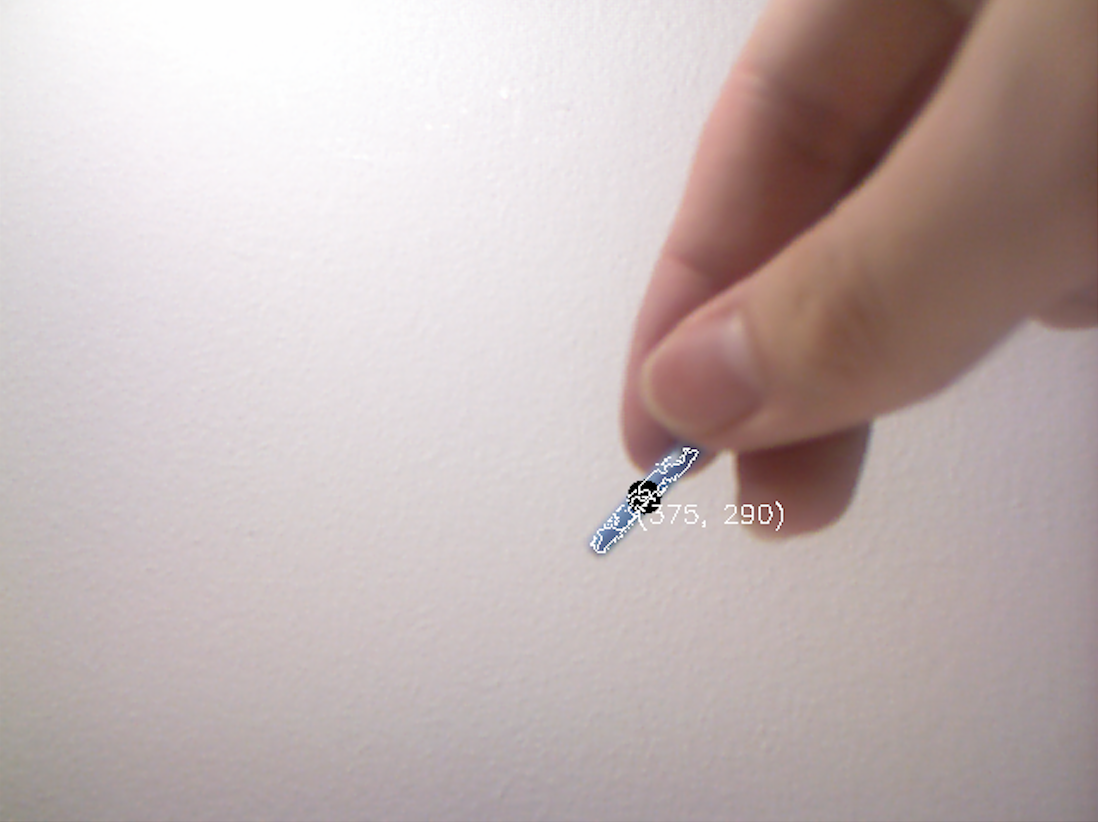
\includegraphics[width = 0.3\columnwidth]{images/4_1.png}
%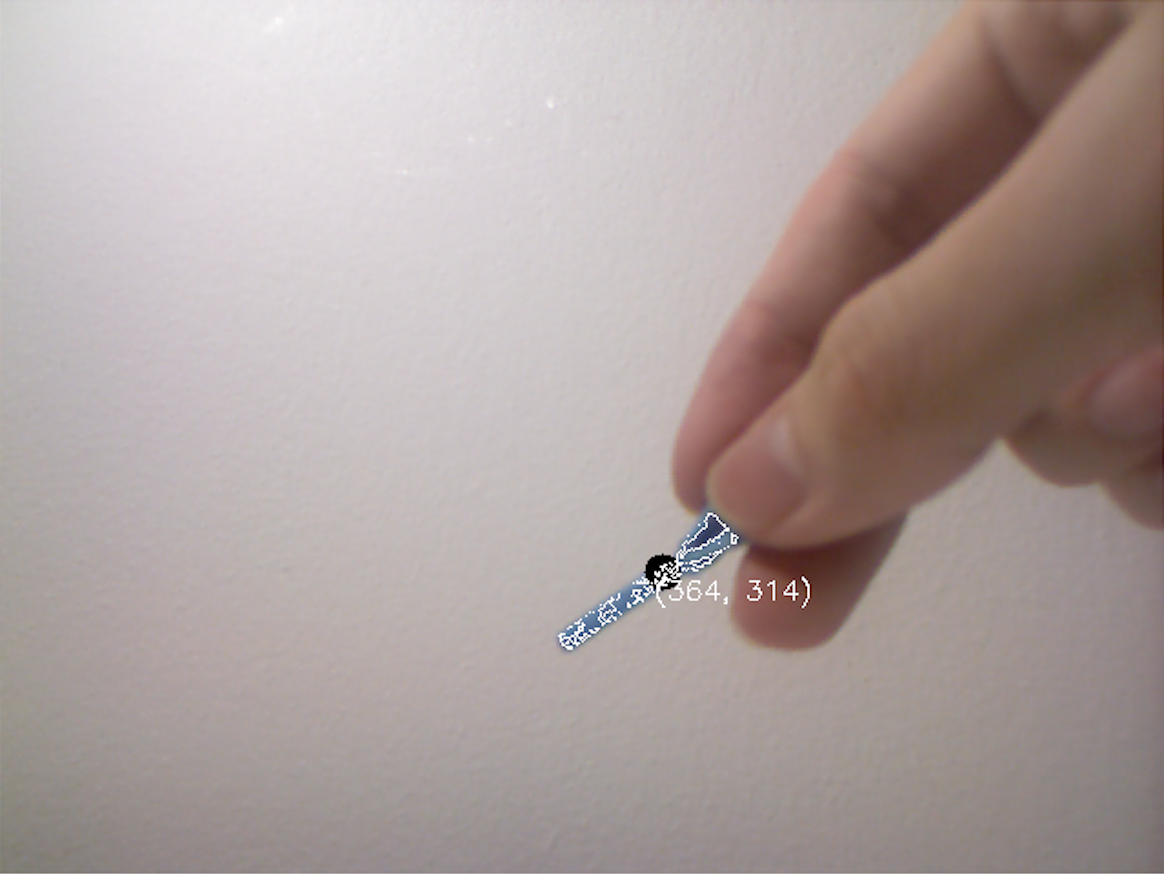
\includegraphics[width = 0.3\columnwidth]{images/5_1.png}
%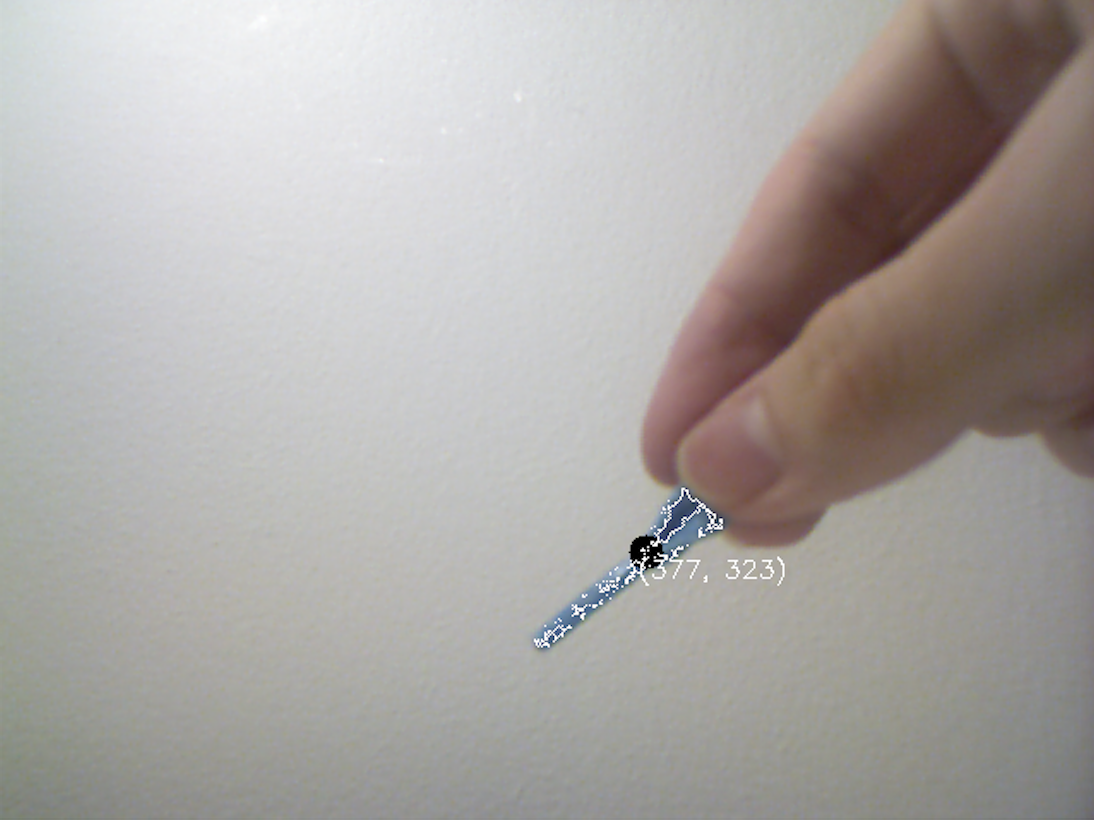
\includegraphics[width = 0.3\columnwidth]{images/6_1.png}
\subfigure[warm light]{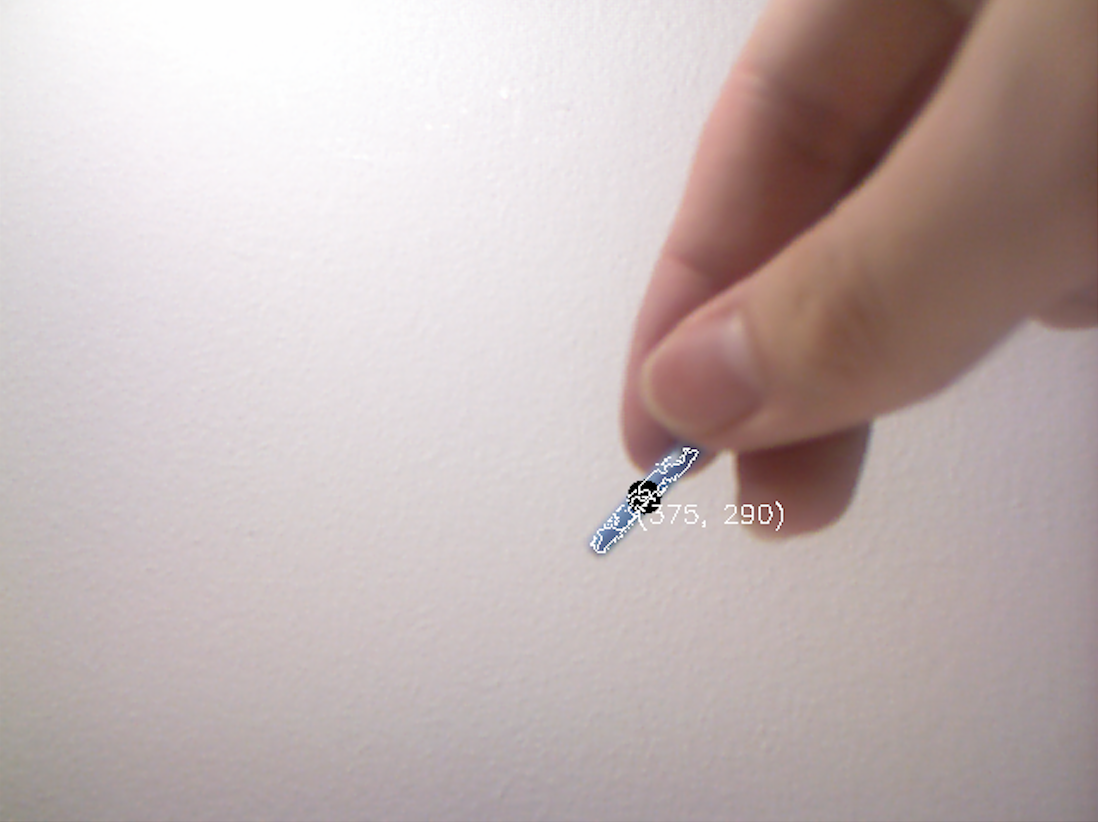
\includegraphics[width = 0.33\columnwidth]{images/4_1.png}}%
\subfigure[normal light]{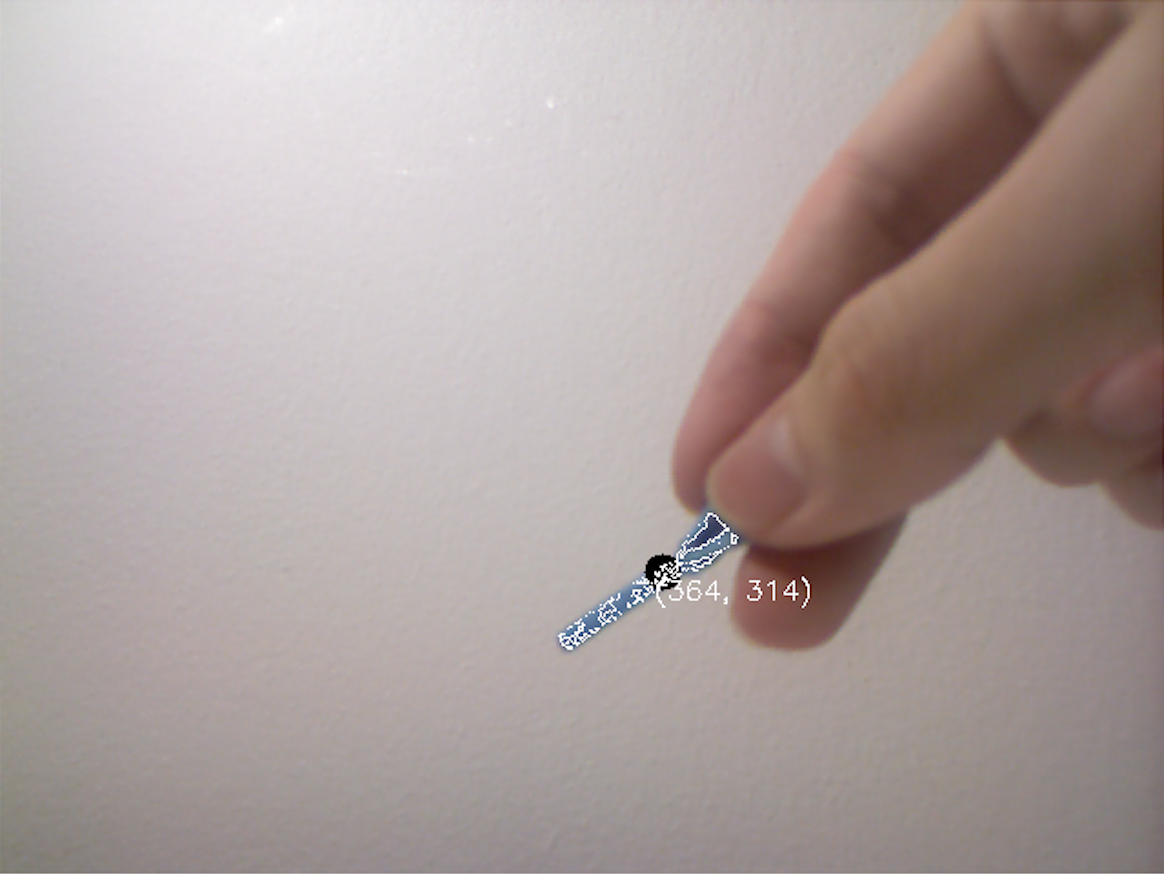
\includegraphics[width = 0.33\columnwidth]{images/5_1.png}}%
\subfigure[cold light]{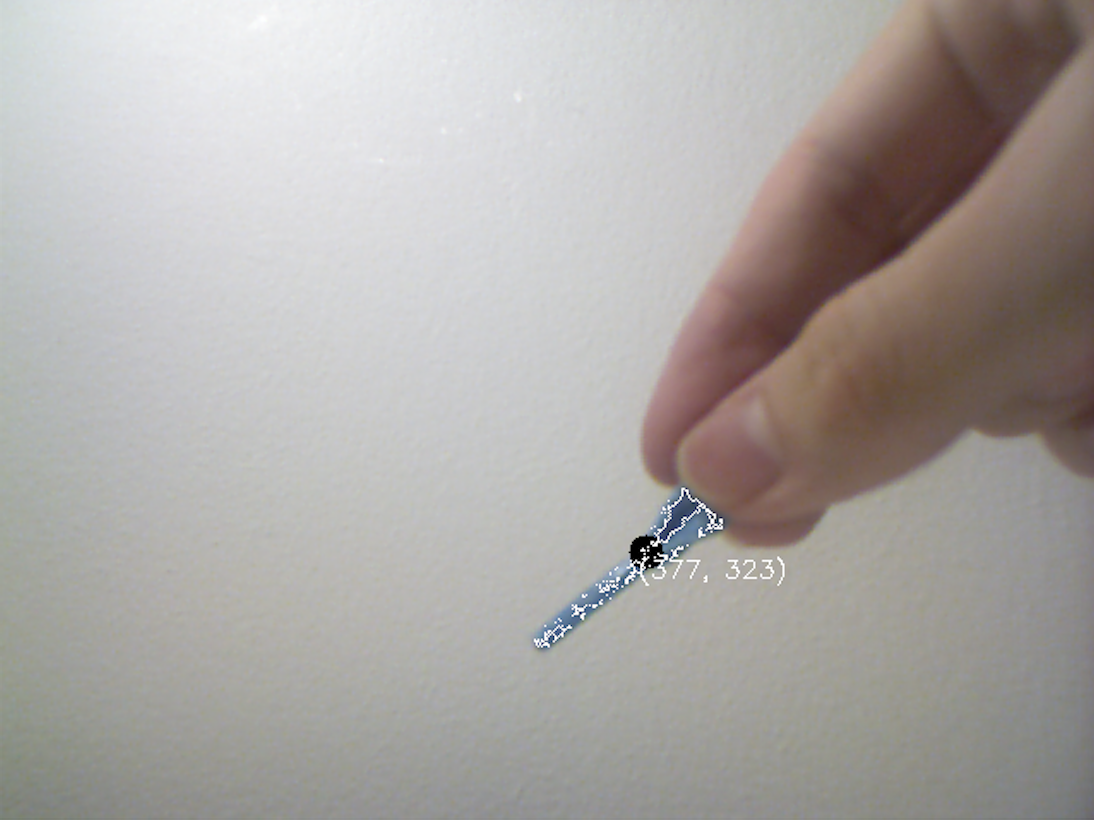
\includegraphics[width = 0.33\columnwidth]{images/6_1.png}}%
\caption{Color detection algorithm testing on a shoelace in different environments}%
\label{shoelace}%
\end{figure}
%--------------------------
When detecting the shoelace or the shoe holes, it is expected that the camera is quite close to them and there will not be any other objects in camera's sight. Also, different lighting conditions will have less influence on the result. This test was carried out in warm light, normal light and cold light. All these test results indicate the color detection can precisely locate the head of a shoelace. 

\begin{figure}[H]
    \centering
    \subfigure[real robot]{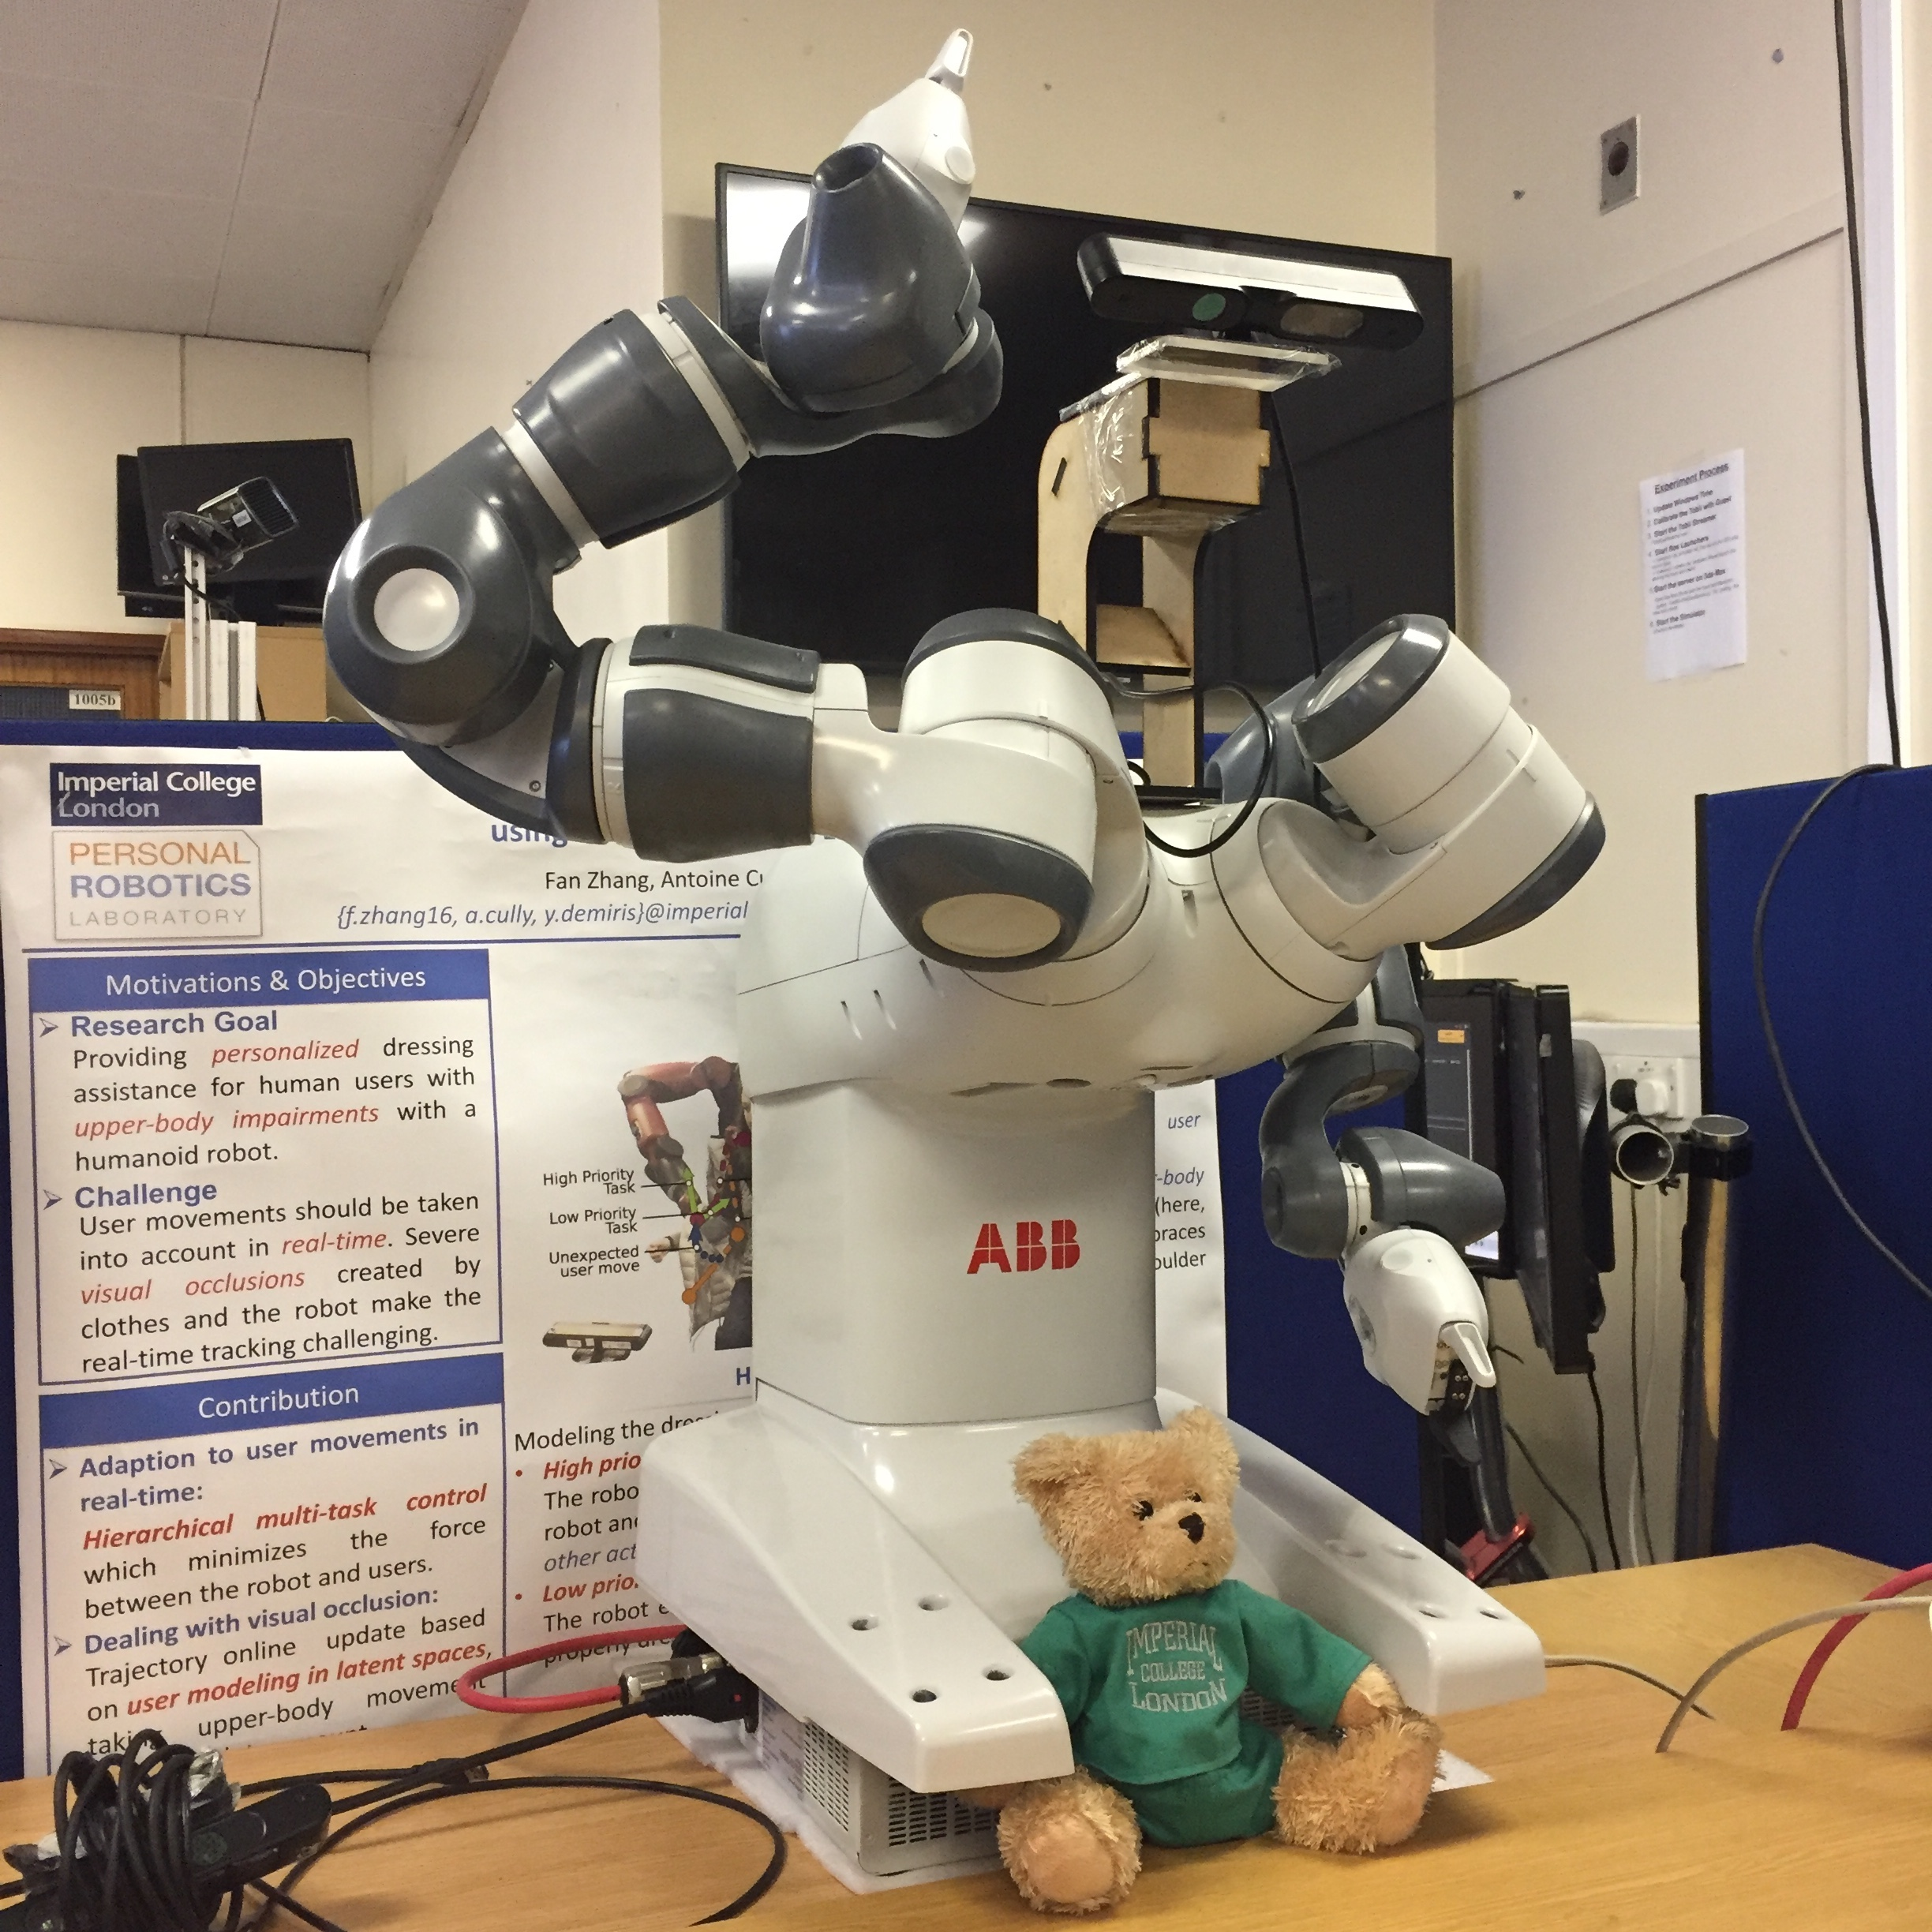
\includegraphics[width = 0.355\columnwidth]{images/yumi_pose.png}}%
    \subfigure[view in Rviz]{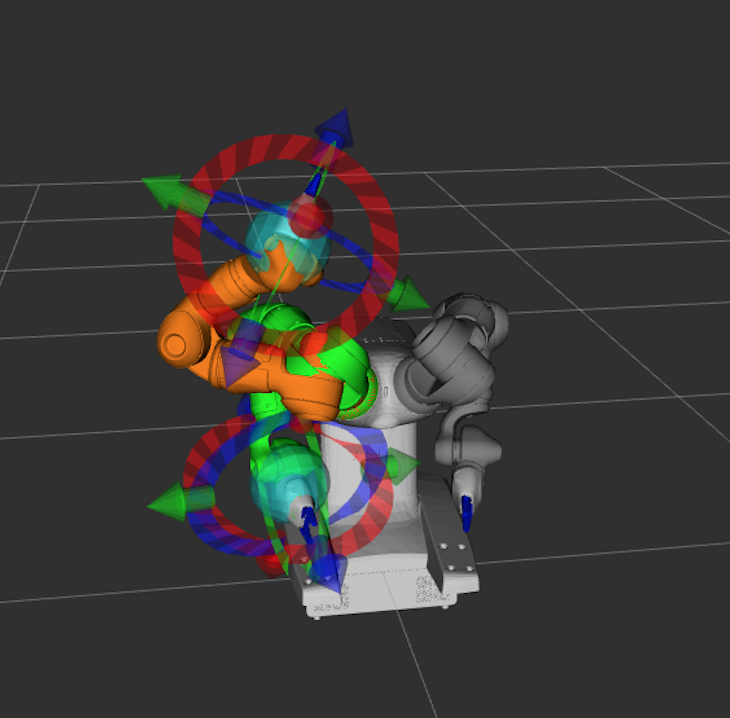
\includegraphics[width = 0.36\columnwidth]{images/rviz_pose.png}}%
    \caption{YuMi motion planning}
    \label{motion}
\end{figure}

In the meanwhile, preliminary motion planning algorithm has been developed using Python, based on OMPL and MoveIt! to control the movements of robot's both arms and grippers. Figure \ref{motion} shows one specific pose and the corresponding view in Rivz. Motion of YuMi has been planned by setting a joint goal, setting a pose goal for end-effector and specifying a Cartesian path directly. All these methods have been tested and they work well.
%Motion can also be planned using Rviz by dragging the green arm (start state) and orange (goal state) to wanted spots.

The main task in the following month is to finish the 3D object localization algorithm using YOLO9000 and color detection, and then combine the vision part with the motion planning part to complete stage one. YuMi's left gripper and gripper cameras have not been successfully tested and need to be checked as soon as possible.

\section{Stage Two and Three}
%breakdown of the work that is to be done in the remainder of the project. 
%Future project work is identified as a set of tasks with chronological order and dependencies.
After successfully achieving the deliverable of stage one, stage two and three will start to be developed. Since planning every single motion is time-consuming, and the motions of pulling shoelace out of a shoe hole are similar each time, I consider to pre-compute several motions for YuMi. I will probably define some fixed poses, e.g., initial pose, the pulling pose (used while pulling the shoelace out), searching pose (while searching for the next shoe hole). For every pose, I will pre-compute a joint trajectory such as from the pulling pose to searching pose. Whenever possible, YuMi uses these trajectories to reach its goal and only checks if collisions exist between it and environment before execution. I suppose this will reduce computational time and let YuMi perform more smoothly. Besides, how to label the order of shoe holes will be further investigated. Research on computer vision and motion planning will be kept carrying on till the end of this project. 


\section{Fallbacks} %%It should also detail fallback positions in case any stage of the development goes wrong. 
If the whole project does not go well or face some particular difficulties, finishing the core project (stage one and two) in time can be considered as a fallback. If the situation is even worse, placing the shoes in a fixed location instead of a random spot to perform these tasks is an alternative. Another possibility might be replacing the shoe with other objects, then using vision and motion planning knowledge to let robot manipulate them.


\section{Uncertainties} %Task risks and uncertainties (of slow completion or non-completion) are discussed.

Stage one and stage two are the core of this project, whose estimated finishing time is the end of March 2019. Therefore, it is supposed that, from April to end of June, there is a two-month buffer period to deal with any uncertainties.